\documentclass[../main.tex]{subfiles}

\begin{document}
\chapter{Results and Discussion}
\label{cha:Results}

% \begin{itemize}
%     \item list assumptsion
%     \begin{itemize}
%         \item that over rl training is a good measure of skill
%         \item that win-rate is a measure of skill?
%     \end{itemize}
%     \item list limitations
%     \begin{itemize}
%         \item 
%     \end{itemize}
%     \item confidence inervals
% \end{itemize}

% \note{binomial confidence intervals \cite{brown_interval_2001}}

In this chapter I present the results of the experiments described in \cref{method:experiments}, and their implications with respect to the research questions from \cref{intro:reserach-qs}.

\section{The effect of going first}
\cref{tab:rule-wr-going-first} shows the results from the first experiment. Games against the random agent do not see significant change as any strategy employed against a random agent will yield high win rates. The increase over the original comparison (\cref{tab:rules-winrates}) is shown in brackets.

\begin{table}[]
    \centering
    \begin{tabular}{@{}llll@{}}
                 & Random & Novice & Intermediate \\
    Random       & 0.0655 (\minus0.0019) & 0.0186 (\pos0.0035) & 0.0111 (\pos0.0000)  \\
    Novice       & 0.9414 (\minus0.0003) & 0.5149 (\pos0.0352) & 0.3421 (\pos0.0190)  \\
    Intermediate & 0.9865 (\pos0.0023)   & 0.6921 (\pos0.0175) & 0.5206 (\pos0.0253)    
    \end{tabular}
    \caption{Win rates table (Row vs. Column) rule based agents where the row is fixed as the starting player. Averaged over 10000 games per pairing. Difference from \cref{tab:rules-winrates} shown in brackets.}
    \label{tab:rule-wr-going-first}
\end{table}

In the match ups between the novice and intermediate agents, each agent when going first saw an increase in their win rate, between 1.75-3.52\%. This shows that going first does increase the win rate of a player as hypothesised in \cref{hyp:going-first}. This holds for players that use a strategy. For the random agent it is unsurprising that there is little to no effect. 

The notable change is in self-play mode where the agent going first increases their win percentage by over 2\%. Since the agents are of the same skill level it shows the impact that going first has. As hypothesised in \cref{hyp:first-overtime} the effect of going first is lessened. The increase of the intermediate agent over the novice agent is smaller than the other way around. I imagine this is because the stronger strategy of the intermediate agent is more significant. 

\cref{fig:going-first-over-time} shows the results of the RL agent going first in self play as it is trained. There is a small increase of ~3\% over the usual 50\% win rate. This stays constant over the course of training. Likewise, \cref{fig:win-rate-vs-int-going-first} plots effects of going first using the intermediate agent and the RL agent as it's trained. 

Both of these plots do not show a significant change of the effect that starting a round has on win-rate as the agent's skill increases. 

\begin{figure}
    \centering
    \begin{subfigure}[t]{0.49\textwidth}
        \centering
        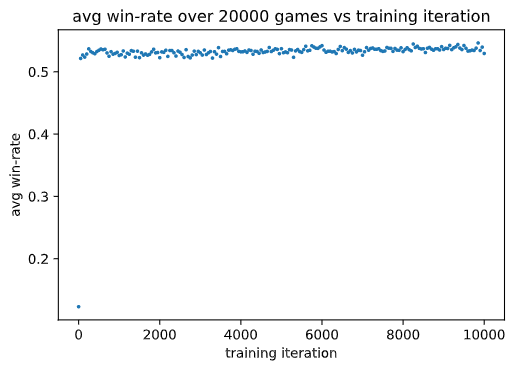
\includegraphics[width=\textwidth,keepaspectratio]{images/results/going_first_over_time.png}
        \caption{Win rate vs Training Iteration in self play when the agent going first is fixed. Every 100th training iteration using 20000.}
        \label{fig:win-rate-going-first}
    \end{subfigure}
    \hfill
    \begin{subfigure}[t]{0.49\textwidth}
        \centering
        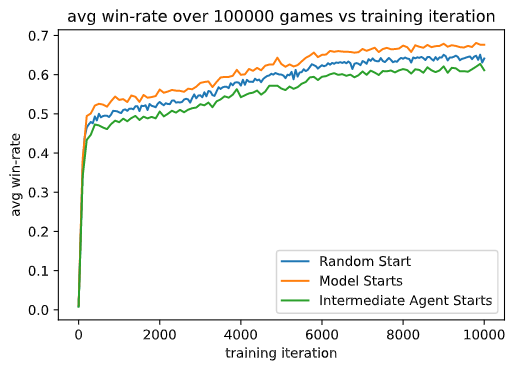
\includegraphics[width=\textwidth,keepaspectratio]{images/results/winrate_vs_int_going_first.png}
        \caption{Win-rate for the model versus the intermediate agent. 20,000 games simulated at every 100th training iteration.}
        \label{fig:win-rate-vs-int-going-first}
    \end{subfigure}
    \caption{Going first over training iteration.}
    \label{fig:going-first-over-time}
\end{figure}


%%%%%%%%%%%%%%%%%%%
%% STARING HANDS %%
%%%%%%%%%%%%%%%%%%%

\section{The effect of starting hands}
\subsubsection{Starting with a specific score}
The first experiments looked at the effect a starting a game with a hand that had a specific total score. \cref{fig:startinghand-winrates} shows the results. There is a clear increase in win rate as initial hand score reduces, to 1 -- as mentioned in \cref{intro:reserach-qs} starting with a hand less than 8 should mean a 99.99\% win chance if the player calls Yaniv straight away. This seems to support \cref{hyp:hand-score}. 

However, as a player's hand score increases past ~40 points their chances of winning increases too. This can be attributed to the fact that there are fewer possible ways of making large scores. This means that a higher value hand is more likely to have a better hand combination in it. There is a clear relationship between the score of a starting hand and its win rate, but it is not linear, and so we must reject \cref{hyp:hand-score}. 

It is worth noting, that the vast majority of the hands are distributed around the 50\% win rate area as shown in \cref{fig:startinghand-probs}. 

\begin{figure}
    \centering
    \begin{subfigure}[t]{0.49\textwidth}
        \centering
        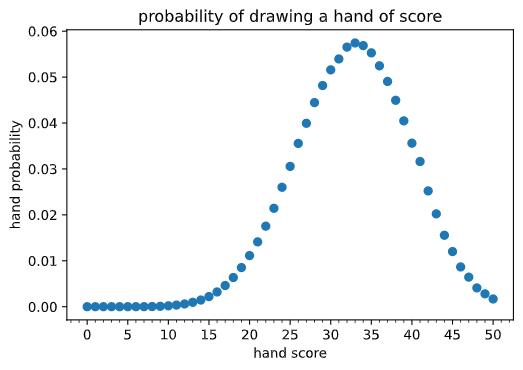
\includegraphics[width=\textwidth,keepaspectratio]{images/results/handscores.png}
        \caption{Frequency of 5 card hand combinations which score. Note that the lowest possible hand score is 6 (4 aces and a two).}
        \label{fig:startinghand-probs}
    \end{subfigure}
    \hfill
    \begin{subfigure}[t]{0.49\textwidth}
        \centering
        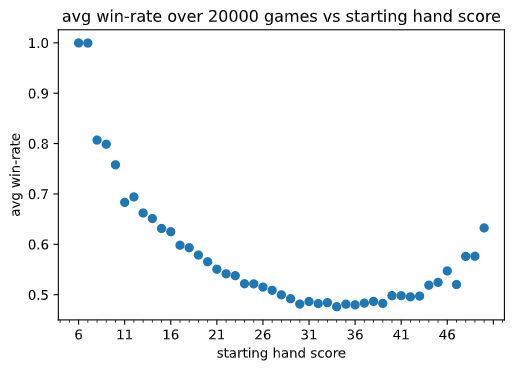
\includegraphics[width=\textwidth,keepaspectratio]{images/results/winrate_handscore.png}
        \caption{Win-rate for a given starting hand score.}
        \label{fig:startinghand-winrates}
    \end{subfigure}
    \caption{Hand score results.}
    \label{fig:handscores}
\end{figure}




\subsubsection{Starting with a specific hand class}

\cref{fig:handclass-vs-self} shows the results of the experiment to test \cref{hyp:hand-class}. Using the intermediate agent as an example, in self play mode there is clear evidence to accept \cref{hyp:hand-class}. The hand classes can be broken down in to 6 categories: 2X, 2X2X, 3X, 3X2X, 4X, 5X (3X2X = 3 card combination + 2 card combination). 2X2X and 3X have similar win rates, then there is a marked increase to 3X2X, again to 4X and again to 5X. 

However, the RL model behaves  differently to the intermediate agent. It's better able to take advantage of 3K2K but at the higher order combinations it does worse. This is understandable considering the frequency of 5S and 4K (shown in \cref{tab:hand-classes}). Since it is unlikely that the agent has encountered situations where it can put down a 5 card straight or 4 of a kind, the agent doesn't know how to deal with these rare occurrences. Unlike the heuristic agent which has the rules that cover these events. Under the limitations of the experiment it is not possible to accept \cref{hyp:hand-class}. It is true for the intermediate rule agent, and perhaps any \textit{good} player. 

% The idea that it is possible to use an RL agent sampled at steps as it trains as a continuous measure of skill may be flawed. 

\cref{fig:handclass-int-vs-model} shows the results when pairing up the intermediate rule agent and RL model. Orange shows when the intermediate agent starts the game with the class, and the RL model has a random hand, the opposite for blue. The baseline win rates are also shown as the dotted line for each agent when starting with random hands, so any increase above that line is positive. 

The shape of the increases over the baseline win rates in \cref{fig:handclass-int-vs-model} is similar to self play mode (a). The advantage gained is amplified for the intermediate agent, since its base win rate was so low against the RL model -- it's still able to win almost 90\% of games when starting with a 5 card straight. Likewise, the effects are dampened somewhat for the RL model, since it already wins over 60\% of the time against the intermediate agent. This goes some way to showing that the effect a starting hand has on your win rate will depend on the baseline win rate -- i.e. the difference in skill between players. 

\begin{figure}
    \centering
    \begin{subfigure}[t]{0.49\textwidth}
        \centering
        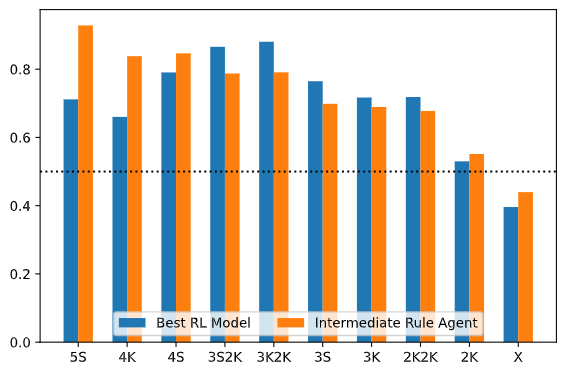
\includegraphics[width=\textwidth,keepaspectratio]{images/results/handclasses.png}
        \caption{Win rates for each hand class. Agents play against themselves for 100,000 games per hand class. The 50\% line is marked, anything above this in an increase.}
        \label{fig:handclass-vs-self}
    \end{subfigure}
    \hfill
    \begin{subfigure}[t]{0.49\textwidth}
        \centering
        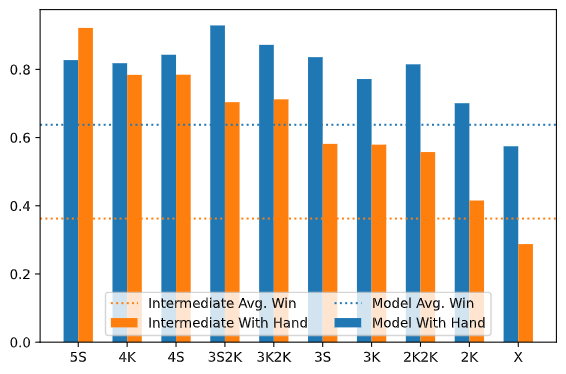
\includegraphics[width=\textwidth,keepaspectratio]{images/results/handclasses_model_vs_rules.png}
        \caption{Hand class win rates for Model vs Intermediate. Along with the baseline win-rate for each (random hands).}
        \label{fig:handclass-int-vs-model}
    \end{subfigure}
    \label{fig:handclass-winrates}
    \caption{Win rates for different hand classes. Uses the intermediate rule agent and the 10,000th iteration of the RL model. Averaged over 100,000 games. The opponent's starting hand is sampled from the deck after generating the starting hand of the given class.}
\end{figure}

\cref{fig:handclass-overtime} displays the results of the final experiment. Using samples of the RL model as it's trained gives an estimation of increasing skill. It quickly picks up on basic strategy, then around iteration 4000 the model starts to get better at 3K, which has the effect of also improving 3K2K. I believe this is where the agent learns to exploit three of a kind, instead of just putting down two cards.

This shows that in order to get the most out of certain hand classes a player must know how to exploit them. This is the essence of \cref{hyp:class-overtime}. As the RL model gathers more in game experience its able to increase its win rate when starting with specific hand classes.

\begin{figure}
    \centering
    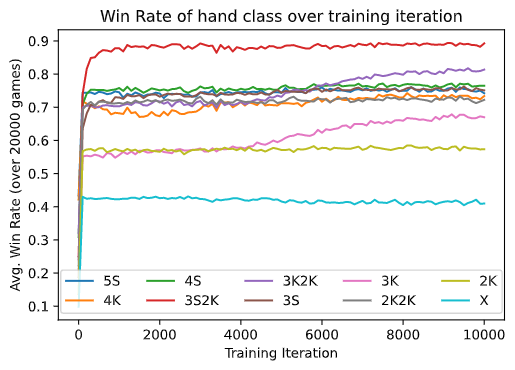
\includegraphics[width=\textwidth,keepaspectratio]{images/results/handclassovertime.png}
    \caption{Win-rate for given class over training iterations.}
    \label{fig:handclass-overtime}
\end{figure}

\section{Limitations and assumptions}
Throughout this project we have used a player's win-rate versus the baseline heuristic agents to determine their skill level. There is a clear reason for this; if an agent wins 50\% of the time against their opponent then they must have the same level of skill. Likewise, if they win 60\% of the time then you can assume they are better. However, there is more to Yaniv, as the score a player loses on is important. If two players have an equally matched win rate (50\%), but one scores less on average when they lose, then they must have more skill. A better measure of performance might be the average round score, that is the loss proportion multiplied by the average losing score. 

% We have also assumed that an RL agent in training can be used as a constantly increasing skill. \note{more}
\end{document}